\chapter[Le transistor]{Le transistor CMOS\\{\it La naissance des 0 et 1}}

\minitoc

\section{Introduction}
Ce chapitre vise à présenter le transistor CMOS de manière très succinte. Plus précisément, nous cherchons à illustrer les étapes successives qui permettent
de passer du Silicium,  l'élément chimique de la table périodique des éléments, à de véritables interrupteurs miniaturisés. Nous passerons sous silence
les capacités d'amplification de ces transistors, ainsi que les équations fondamentales qui en régissent le fonctionnement. On pourra se reporter à différents
ouvrages comme \cite{Weste2010} ou \cite{Ngo2012} pour plus de détails, y compris concernant les {\it process} de fabrication, également survolés ici.

\section{Silicium et dopage}
Le silicium  est l'élément chimique dénoté {\it Si} dans la table périodique des éléments, de numéro atomique $14$.
Sa forme cristallographique présente un double réseau (identique à celui du diamant), décalés l'un de l'autre du quart de la diagonale principale. Sur chacun des réseau les atomes de silicium se situent au sommet d'un cube, ainsi que sur chacune des face de ce cube (il est dit ``cubique face centrée'').

\begin{figure}[htb]
\begin{center}
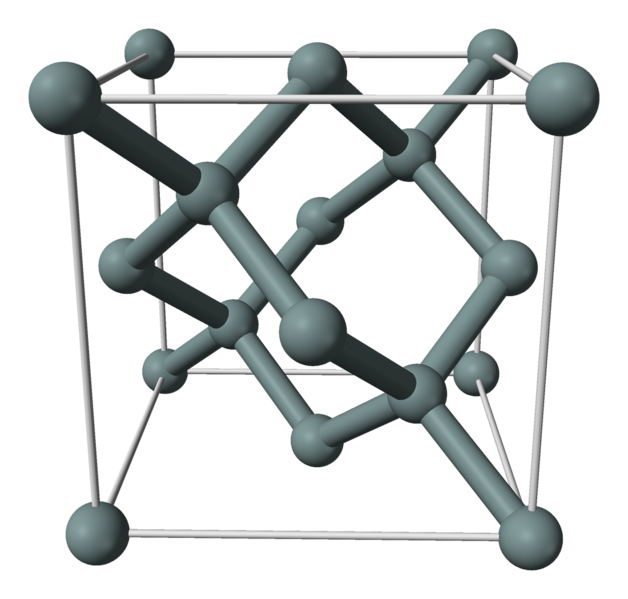
\includegraphics[scale=0.15]{figures/double_fc.png}
\caption{La maille élémentaire du cristal de silicium}
\end{center}
\end{figure}

Ses propriétés physico-chimiques en font un semi-conducteur : sa conductivité électrique est notamment bien inférieure à celle d'un métal. Dans le double réseau, chaque atome de silicium peut être considéré comme au centre d'un tétraèdre, chacun des atomes auquel il est lié se trouvant sur un des quatre sommets du tétraèdre. Les liaisons covalentes sont très solides et permettent la formation d'un cristal parfait. Tous les électrons étant utilisés dans les liaisons, aucun n'est disponible pour permettre le passage d'un courant électrique, du moins aux températures très basses ; le cristal présente une résistivité assez élevée. Lorsque la température s'élève, sous l'effet de l'agitation thermique, des électrons réussissent à s'échapper et participent à la conduction. Ce sont les électrons situés sur la couche la plus éloignée du noyau qui s'impliquent dans les liaisons covalentes. Dans le cristal, ces électrons se situent sur des niveaux d'énergie appelée bande de valence. Les électrons qui peuvent participer à la conduction possèdent des niveaux d'énergie appartenant à la bande de conduction. Entre la bande de valence et la bande de conduction peut se situer une bande interdite. Pour franchir cette bande interdite l'électron doit acquérir de l'énergie (thermique, photon...). Pour les isolants la bande interdite est quasi infranchissable, pour les conducteurs elle est inexistante. Les semi-conducteurs ont une bande interdite assez étroite.\\

\begin{figure}[htb]
\begin{center}
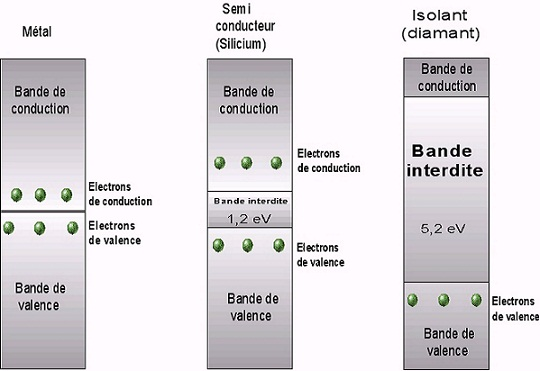
\includegraphics[scale=1.3]{figures/bande-interdite-valence-et-conduction-copie.png}
\caption{Bande de valence et de conduction de différents types de matériaux}
\end{center}
\end{figure}

L'atome qui a perdu un électron devient un ion positif et le trou ainsi formé peut participer à la formation d'un courant électrique en se déplaçant.
Dans un cristal pur, à température ordinaire, les électrons libres sont malgré tout extrêmement rares - de l'ordre de 3 pour $10^{13}$ atomes !
Si l'électron libre est capté par un atome, il y a recombinaison. Pour une température donnée ionisation et recombinaison s'équilibrent ; la résistivité diminue quand la température augmente.
Un semi-conducteur dont la conductivité ne doit rien à des impuretés est dit {\it intrinsèque}.\\

Lors de la formation du cristal de silicium il suffit d'introduire une infime quantité d'impuretés sous la forme d'atomes d'aluminium (possédant seulement 3 électrons sur leur couche externe) pour que le nombre de trous dans le cristal augmente considérablement. Le cristal est dit dopé et comme les porteurs de charges majoritaires sont des trous, positifs, le cristal est dit dopé P. Les électrons libres qui correspondent à la conductivité intrinsèque sont
appelés porteurs minoritaires.
Si un électron est arraché d'un atome voisin et vient combler le trou, tout se passe comme si c'était le trou qui s'était déplacé.
On peut également doper le cristal avec des impuretés pentavalentes (atomes possédant 5 électrons sur leur couche externe),
comme l'arsenic ou l'antimoine. On se retrouve alors avec un électron supplémentaire, donc libre. Les porteurs de charges majoritaires
sont alors de polarité négative, le cristal est dit dopé N. Les porteurs de charge minoritaires sont dans ce cas les trous (positifs)
de la conductivité intrinsèque.\\

\begin{figure}[htb]
\begin{center}
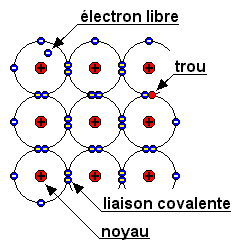
\includegraphics[scale=0.5]{figures/cristal.png}
\caption{Présence des différents porteurs de charge}
\end{center}
\end{figure}

Un atome pentavalent comme l'arsenic possède 5 électrons sur sa couche externe. En tant qu'impureté dans un cristal de silicium
(tétravalent) il fournit un électron au cristal. Il est dit atome donneur.
Si l'impureté est un atome trivalent (3 électrons sur sa couche externe, comme le bore ou l'indium) il est dit atome accepteur car il va
capter un électron et générer un trou. Les porteurs majoritaires sont beaucoup plus nombreux que les porteurs minoritaires ($10^6$ à $10^{12}$ fois
plus nombreux).\\

\paragraph{En résumé} Le fait d'introduire en très faible quantité des impuretés (opération appelée dopage) dans un cristal de semi-conducteur améliore
fortement la conductivité du cristal. Si un cristal de germanium ou de silicium a reçu des impuretés pentavalentes (arsenic, phosphore,
antimoine) il devient un semi-conducteur à conductivité N (ex: silicium N).
Un cristal de germanium dopé par des impuretés trivalentes (indium, gallium, bore) devient un semi-conducteur P.

\section{Jonction PN}
Une jonction entre des cristaux de silicium de type {\it p} et de type {\it n} est appelé une {\bf diode}. Cette jonction est le simple rapprochement
de ces deux cristaux. Ses propriétés sont particulièrement remarquables.\\

\begin{figure}[htb]
  \begin{center}
    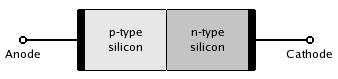
\includegraphics[scale=0.6]{figures/PN_Junction_Open_Circuited.png}
    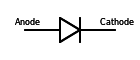
\includegraphics[scale=0.8]{figures/Diode_symbol.png}
    \caption{Jonction PN ou diode}
  \end{center}
\end{figure}

\begin{itemize}
  \item Lorsque la tension sur le semi-conducteur de type p, appelée anode, est supérieure à celle la tension sur la partie dope n (cathode), la diode est polarisée en direct et le courant circule.
  \item Lorsque la tension d'anode est inférieure ou égale à la tension de cathode, la diode est polarisée en inverse et très peu de courant circule.
\end{itemize}

\begin{figure}[h!bt]
  \begin{center}
    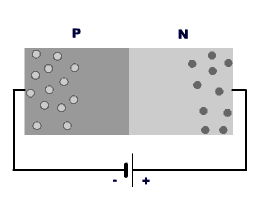
\includegraphics[scale=0.4]{figures/Diffusion3.png}
    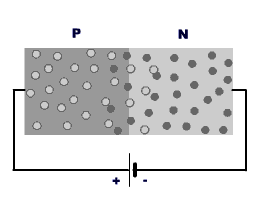
\includegraphics[scale=0.4]{figures/Diffusion4.png}
    \caption{Jonction PN passante ou bloquée en fonction de la polarisation.}
  \end{center}
\end{figure}

Ce dipôle est aussi appelé diode de redressement car il est utilisé pour réaliser les redresseurs qui permettent de transformer le courant alternatif en courant continu.

\section{Transistor MOS}

Le transistor est un composant électronique qui a deux utilités majeures : il permet d'{\bf amplifier un courant ou une tension}, ou il peut être utilisé comme un {\bf interrupteur commandable en courant ou en tension}. Dans la suite, nous n'utiliserons que cette seconde capacité. Il existe deux catégories de transistor :
\begin{itemize}
\item les transistors bipolaires, constitués par la succession de trois zones dopées PNP ou NPN.
\item les transistors MOS, qui représentent désormais plus de 85\% du marché.
\end{itemize}


%% \begin{figure}[htb]
%% \begin{center}
%% 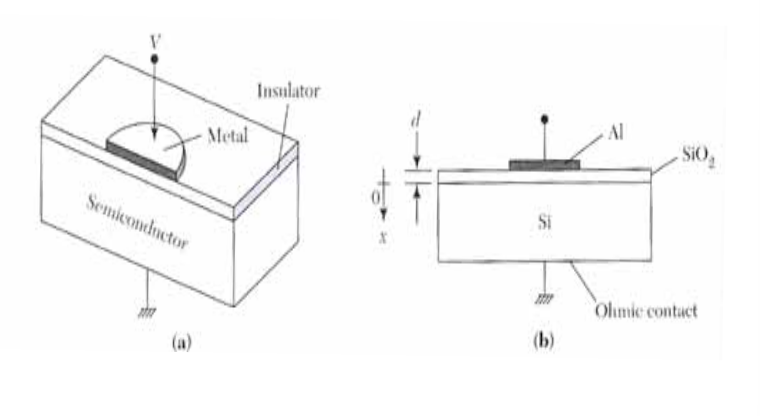
\includegraphics[scale=0.3]{figures/MOS.png}
%% \caption{Structure MOS}
%% \end{center}
%% \end{figure}

%http://www.etudes.ecp.fr/physique/illustrations/jonction_PN.htm#debut

La figure suivante présente la structure d'un tel transistor, ici de type $n$.

\begin{figure}[htb]
\begin{center}
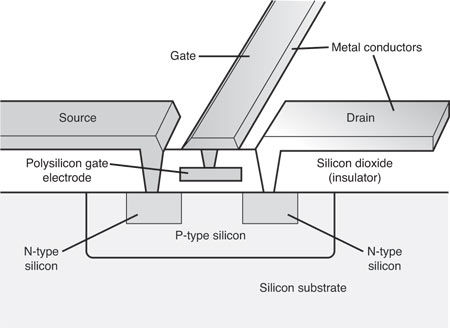
\includegraphics[scale=0.6]{figures/n-MOS_2.png}
\caption{Transistor $n-MOS$}
\end{center}
\end{figure}

Un tel transistor présente une structure en sandwich :
\begin{itemize}
\item une grille (gate) conductrice (généralement du métal ou du silicium polycristallin)
\item une couche isolante (oxyde de silicium $SiO_2$)
\item le substrat de silicium, dont la tension est généralement à la masse.
\item deux zones dopées de manière identique (ici dopées $n$), appelées source et drain.
\end{itemize}

Ces structures sont fabriquées en utilisant une série d'étapes de traitements chimiques impliquant l'oxydation
du silicium, introduction sélective de dopants (impuretés), le dépôt et la gravure de fils métalliques
et des contacts. Tout ceci à l'échelle nanométrique...La complexité de ces traitements justifie le coût très élevé des usines ({\it fab} ou {\it fonderie}) liées à
l'industrie du semiconducteur. L'entreprise taiwanannaise TSMC, leader mondial, a annoncé en 2017 que le coût de son usine permettant des gravures
à 3 nanomètres lui coûterait plus de 20 milliards de dollars. Sa capitalisation boursière était de 173 milliards de dollars fin 2018
\footnote{Chiffre qui dépasse celui d'Intel, mais reste loin de celui de Facebook (500 Milliards) ! Toutefois, pouquoi comparer ce qui n'est guère
comparable : TSMC fait partie d'une industrie "lourde" et stable. Pour mémoire,
Facebook a perdu 114 Milliards de dollars dans la seule journée du 26 juillet 2018, soit 20\% de sa valeur boursière.}.

Comme on peut l'observer, un transistor $n-MOS$ est construit à partir d'un substrat $p$ et de deux régions dopées de type $n$ (c'est l'inverse pour un transistor de type $p$). La grille permet de  contrôler le courant qui circuit entre la source et le drain. Dans le cas d'un nMOS, le substrat est à la masse : par conséquent les jonctions p-n entre les source-substrat et drain-substrat sont polarisées en inverse. Si la grille est également à la masse, aucun courant ne circule entre les deux jonctions : le transistor est non-passant, ou fermé, ou ``OFF''.

Si on élève la tension de la grille, un champ électrique se crée, qui attire les électrons libres sous la couche isolante. Si cette tension est suffisamment élevée le nombre d'électrons dépasse le nombre de trous : une région, appelée ``canal'' se crée, qui se comporte comme un semiconducteur de type $n$, alors que le substrat initial est $p$ ! Un chemin s'établit pour les électrons entre la source et le drain : le transistor devient passant. Il est ouvert ou ``ON''. Pour les pMOS, la situation est exactement opposée.\\

La tension ``suffisante'' est appelée VDD et représente la valeur logique $1$ dans les circuits numériques. Dans les années 70 et 80, VDD valait traditionnellement $5$ volts.
Plus récemment, les transistors ne pouvant supporter de telles tensions, VDD a été réduit à $3.3V$, puis $1.8V$ etc...La tension appelée VSS (ou ground) représente quant à elle la valeur logique $0$. Elle vaut normalement $0$ volts.\\

En simplifiant le mécanisme à l'extrême, les transistors MOS peuvent être vus comme des interrupteurs ON-OFF.
Lorsque la grille d'un transistor nMOS est 1, le transistor est OFF et il existe un chemin de conduction entre source et drain.
Lorsque la grille est à 0, le transistor est OFF et pratiquement aucun courant ne circule entre la source et le drain.
Le transistor pMOS fonctionne à l'opposé, étant ON lorsque la grille est à 0 et OFF lorsque la tension de grille est 1.

\begin{figure}[htb]
\begin{center}
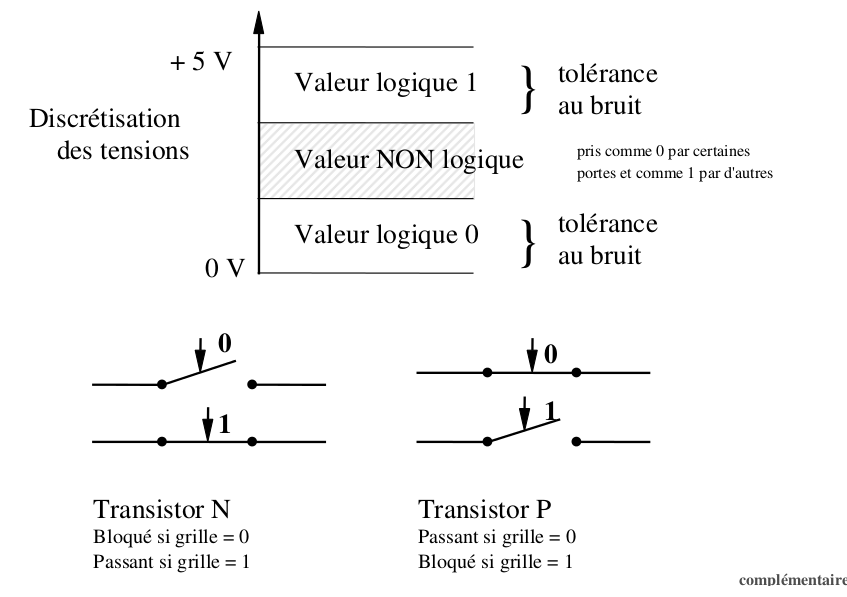
\includegraphics[scale=0.4]{figures/complementaire_1.png}
\caption{CMOS}
\end{center}
\end{figure}

\section{MOS complémentaires}

\paragraph{Principe}
Nous sommes désormais dotés de deux types de transistors. Technologiquement, il a longtemps été question de ne réaliser les circuits numériques à l'aide d'un seul type de transistor (N {\bf ou} P). Mais la technique qui sort largement vainqueur est la logique complémentaire CMOS. Elle consiste à utiliser de manière duale les transistors P {\bf et} N, dans le but de réaliser une fonction logique. Les transistors P sont utilisés pour tirer à 1 et les transistors N pour tirer à 0. Il n'y a pas de perte de seuil. Pour associer ces deux types de transistors, les techniques de dépôts micro-électroniques deviennent plus complexes : il faudrait être à même de
présenter deux substrats différents : un substrat P "collé"" à un substrat N ! Ce n'est pas ce qui est fait technologiquement : en réalité,
on réalise plutôt une zone N sur un substrat P, comme représenté sur la figure \ref{cmos1}.

\begin{figure}[htb]
\begin{center}
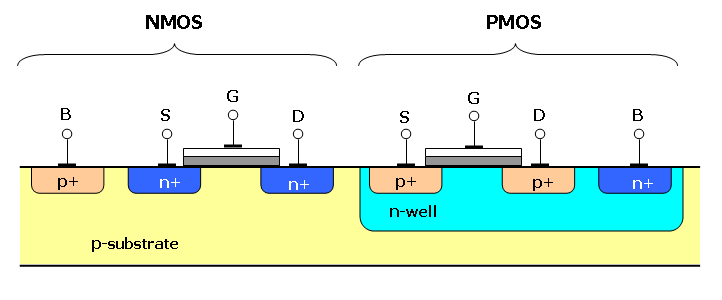
\includegraphics[scale=0.4]{figures/Cmos_impurity_profile.PNG}
\caption{Transistor $C-MOS$}
\label{cmos1}
\end{center}
\end{figure}

\paragraph{Inverseur CMOS}

A titre de premier exemple, considérons le cas d'un {\it inverseur} CMOS sur la figure \ref{cmos2}. On voit qu'il est constitué de deux transistors : la source du transistor P est l'alimentation (5 volts ici),  tandis que celle
du transistor N est la masse (0 V). Ils sont assemblés par leur drain commun et commandés par une entrée (gate) commune.
Lorsque la tension appliquée à l'entrée vaut 0, le transistor P est passant, tandis que le transistor
N est bloqué : la tension issue de l'alimentation se retrouve en sortie. C'est ainsi que l'on a inversé le 0 en 1.
L'inverse s'applique dans le cas d'une tension d'entrée égale à 5 Volts : on transforme le 1 en 0.

\begin{figure}[htb]
  \begin{center}
    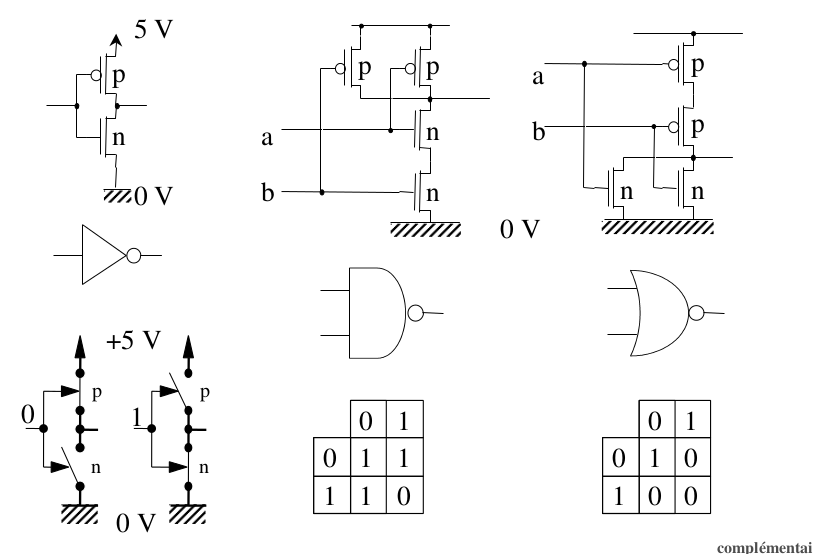
\includegraphics[scale=0.4]{figures/complementaire_2.png}
    \caption{Inverseur logique, porte Nand2 et Nor2 en technologie CMOS}
    \label{cmos2}
  \end{center}
\end{figure}

\paragraph{Principe de dualité}

C'est donc par un montage judicieux, rassemblant deux transistors dopés différemment, que se réalise la fonction d'inversion logique.
La même figure \ref{cmos2} montre que cet assemblage peut se généraliser en réalisant {\it deux réseaux duaux} de transistors P et N.
Par exemple, une porte logique NAND, à deux entrées, se réalise en mettant deux transistors P en {\it parallèle}, alors que les transistors N sont en {\it série}.
Cett dualité se généralise à toutes les fonctions logiques complexes (fig \ref{cmos3}).

\begin{figure}[htb]
  \begin{center}
    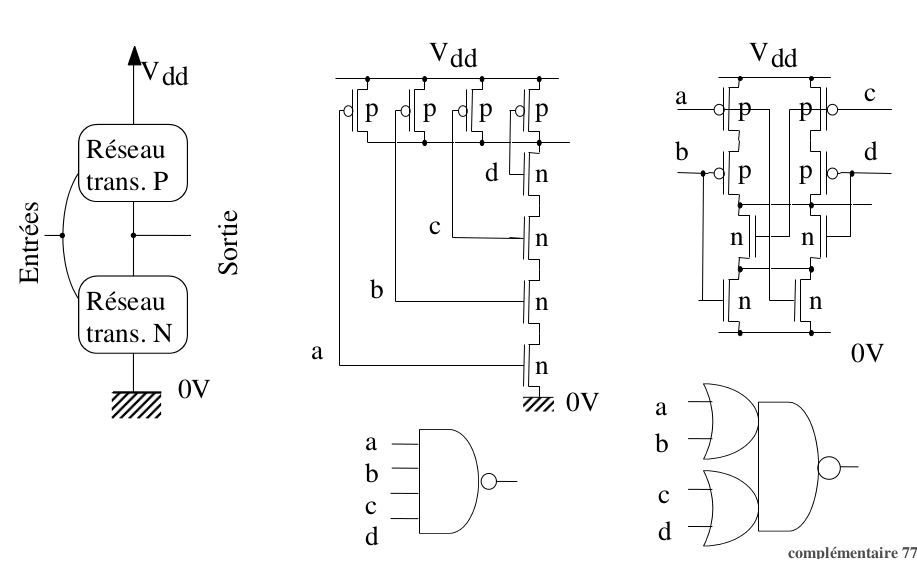
\includegraphics[scale=0.4]{figures/complementaires_2.png}
    \caption{Principe de dualité des réseaux P et N pour des portes logiques complexes}
    \label{cmos3}
  \end{center}
\end{figure}

\section{Niveaux d'abstraction}

\paragraph{De la porte logique au masque métré}
\begin{figure}[htb]
  \begin{center}
    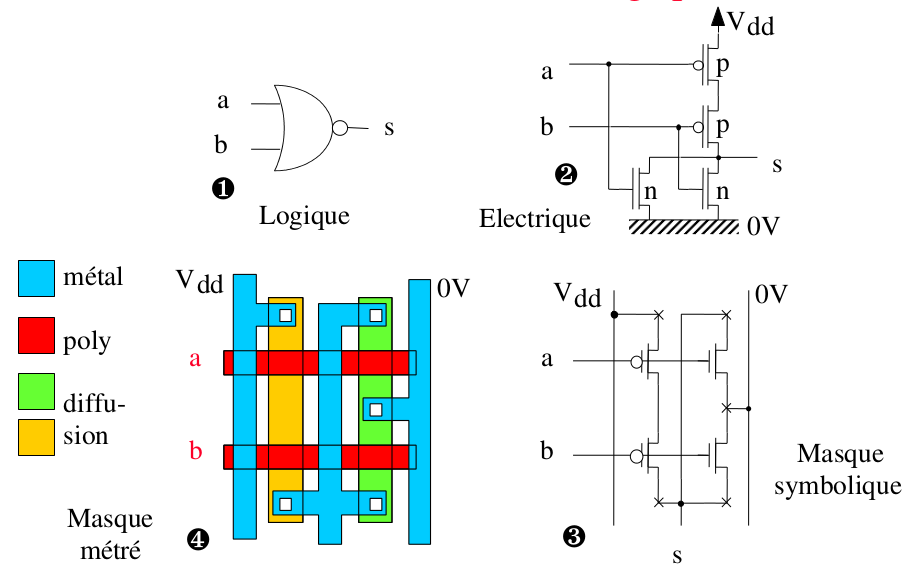
\includegraphics[scale=0.4]{figures/vues_4.png}
    \caption{De la port logique Nor2 au masque métré}
  \label{vues}
  \end{center}
\end{figure}

La montée en abstraction suggérée jusqu'ici, nous faisant passer du silicium à des transistors, puis des premières portes logiques, est illustrée sur la figure \ref{vues}, {\it à rebours} :
le microélectronicien qui souhaite une porte logique (ici un NOR2) devra passer par :
\begin{enumerate}
  \item une décomposition en réseaux P et N de transistors "abstraits", c'est-à-dire affranchis de toute contrainte physique de réalisation. C'est une  sorte de "plan" d'architecte.
  \item un masque symbolique, où l'on dispose soigneusement les équipotentielles de manière géométrique.
  \item un masque métré, où la nature physique des équipotentielles est indiquée (métal, polysilicium etc), ainsi que leur métrage exact. Ce métrage doit respecter des contraintes de {\it layout} (disposition)
  physique précis : certaines zones doivent ne pas s'approcher trop près d'autres région etc...
\end{enumerate}

Ce dernier masque métré reste dessiné dans le plan. Charge à des ordinateurs de calculer leurs dispositions exactes en trois dimensions...Le schéma \ref{cmos4} expose la complexité de
l'enchevêtrement de ces canaux, pour quelques transistors seulement...

\begin{figure}[htb]
  \begin{center}
    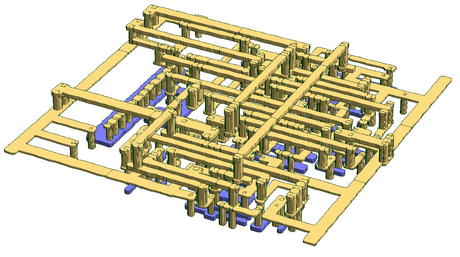
\includegraphics[scale=0.4]{figures/enchevetrement.png}
    \caption{Représentation 3D d'un assemblage de transistors en microélectronique (substrat unique)}
    \label{cmos4}
  \end{center}
\end{figure}

\paragraph{De la porte logique vers le système embarqué}

En 1983, Gajski et Kuhn ont proposé un schéma \ref{gajski} résumant les différentes abstractions d'un système embarqué. Il se présente comme un "Y", dont les trois axes sont :
\begin{itemize}
  \item le comportement du système, vu à différents niveaux d'abstractions
  \item la structure du système, vue à différents niveaux d'abstractions
  \item la géométrie du système, vu à différents niveaux d'abstractions
\end{itemize}

\begin{figure}[htb]
  \begin{center}
  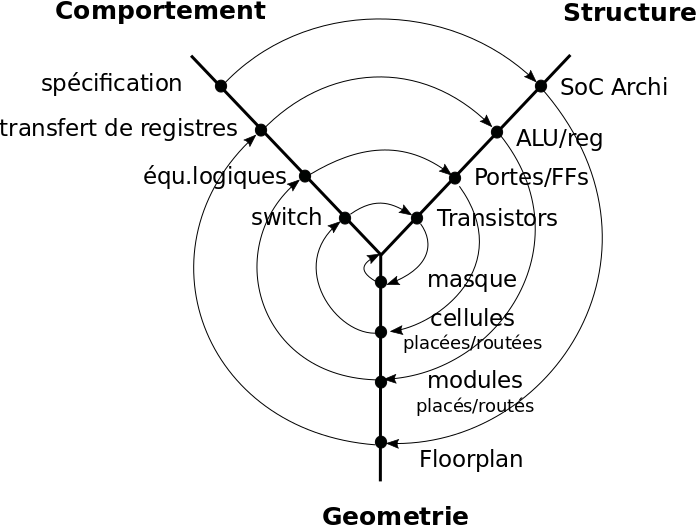
\includegraphics[scale=0.4]{figures/ychart.png}
  \caption{"Y" de Gajski-Kuhn (1983)}
  \label{gajski}
  \end{center}
\end{figure}

La conception d'un "système sur puce" est représenté comme la
succession d'activités d'ingénierie, qui font systèmatiquement passer d'un niveau comportemental à une structure, puis à un niveau géométrie.
Cette succession se répéte en spirale, jsqu'à aboutir à un système réalisé.

Au final, on pourra se satisfaire du schéma \ref{abstractions} qui illustre un sous-ensemble de ces abstractions d'un système.

\begin{figure}[htb]
\begin{center}
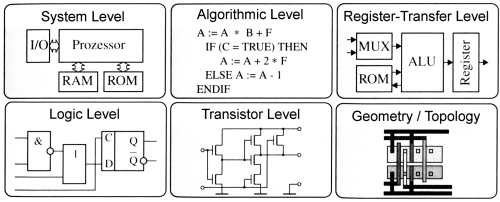
\includegraphics[scale=0.4]{figures/abstractions.png}
\caption{Six vues différentes d'une même système numérique}
\label{abstractions}
\end{center}
\end{figure}

%\section{Equations du transistor MOS en petit signal}

%\section{Technologies microélectroniques}
\section{Numérique versus Analogique}

Nous avons passé sous silence et tenu pour acquis les avantages des circuits numériques sur les circuit analogiques. Ces derniers
ne sont désormais plus utilisés qu'aux interfaces d'un système numérique : pour capter des signaux physiques, pour les amplifier ou les débruiter, etc.
L'Electronique analogique garde tout son intérêt dans le domaine des capteurs, au plus proche de ce monde physique. Mais l'essentiel des traitements effectués
sur le signal se fait par la suite dans un système totalement numérique. En dehors des traitements dédiés, la notion d'ordinateur analogique a totalement disparue, au profit
des ordinateurs que l'on connait depuis longtemps.

La suprémacie du numérique sur l'analogique provient principalement de sa précision maîtrisée : tous les traitements donnent des valeurs exactes, avec une fidélité absolue.

La figure \ref{comparaison} liste quelques uns des avantages et inconvénients des deux Electroniques.

  \begin{figure}[htb]
    \begin{center}
    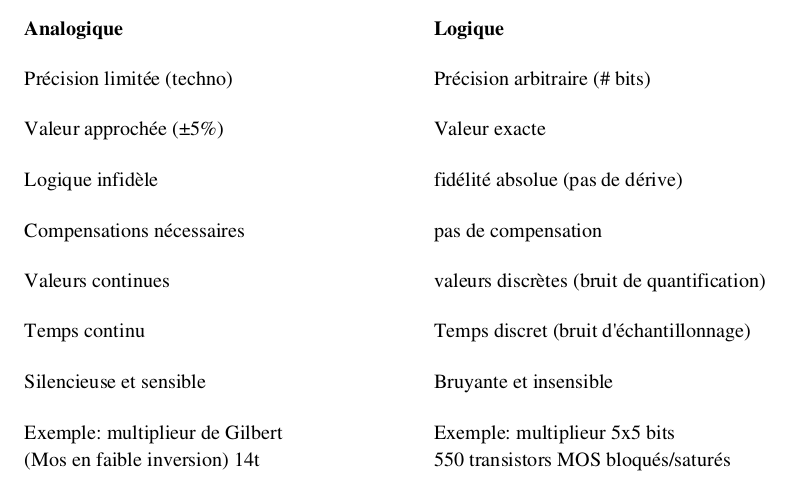
\includegraphics[scale=0.4]{figures/avantages.png}
    \caption{Electronique Analogique et Numériques comparées}
    \label{comparaison}
    \end{center}
  \end{figure}

\section{Conclusions}

Ce chapitre se veut court, car l'ENSTA-Bretagne n'entend pas former des spécialistes de la micro-électronique, ni de la nano-électronique.
Je vous invite toutefois à ne pas perdre de vue, à travers vos lectures, les avancées probables dans le domaine : les progrès de la physique théorique
et appliquée nous apporterons très certainement des révolutions à la hauteur de celles que nous avons vécu dans les années 70. A titre d'exemple, en 2017,
l'ordinateur quantique est en vue ! les promesses seront-elles tenues ?
On peut de même inciter à garder un oeil critique sur les techniques numériques : le tableau suivant compare les avantages et inconvénients de l'électronique
analogique et numérique : comme on peut le voir le numérique se révèle bourré de défauts (exemple : il est plus compliqué de réaliser des opérations arithmétiques,
il est très bruyant,...).
